

\chapter{Reeksen}
\section{Definities}
Rij [$a_n$] = $a_1, a_2, ..., a_n, ...$ met $a_n$ de algemene term.

$$
	[a_n] =
	\begin{cases}
		\hbox{convergent als }  \lim\limits_{n\to\infty} a_n \in \mathbb{R}              \\
		\hbox{divergent naar } \infty \hbox{ als } \lim\limits_{n\to\infty} a_n = \infty \\
		\hbox{divergent als } \lim\limits_{n\to\infty} a_n = ?
	\end{cases}
$$

\example{
	$$\big[\ln(\frac{1}{n})\big]$$
}{
	$$\lim\limits_{n\to\infty} \ln(\frac{1}{n}) = \ln(0^+) = -\infty$$
	Dus divergent naar $-\infty$.
}
\example{
	$$\big[(1 - \frac{1}{n})^n\big]$$
}{
	$$\lim\limits_{n\to\infty} (1 - \frac{1}{n})^n = 1^\infty$$
	Dit is een onbepaaldheid. We maken gebruik van het getal $e$.
	$$=\lim\limits_{n\to\infty} \bigg(1 + \big(-\frac{1}{n}\big)\bigg)^{n(-1)} = e^{-1}$$
	Dus convergent.
}
\example{
	$$2, -1, \frac{1}{2}, -\frac{1}{4}, ..., ...$$
}{
	Bepaal de algemene term: $a_n = 2\bigg(-\frac{1}{2}\bigg)^{n - 1}$
	$$\lim\limits_{n\to\infty} 2\bigg(-\frac{1}{2}\bigg)^{n - 1} = 2\cdot0 = 0$$
	Dus convergent.
}
\example{
	$$[(-2)^n]$$
}{
	$$[(-2)^n] = -2, 4, -8, 16, -32, ...$$
	De laatste term is ofwel positief ofwel negatief. De limiet bestaat niet dus deze reeks is divergent.
}

\section{Hoofdeigenschappen}
Een stijgende rij naar boven begrensd is convergent. Een dalende rij naar onder begrensd is convergent.

In symbolen:

$$a_n \uparrow, \forall n \quad a_n \leq b \rightarrow \hbox{ convergent}$$
$$a_n \downarrow, \forall n \quad b \leq a_n  \rightarrow \hbox{ convergent}$$

\example{
	$$\bigg[\frac{2n - 1}{n}\bigg]$$
}{
	Als $n$ stijgt zal $\frac{1}{n}$ dalen. $2 - \frac{1}{n}$ stijgt dus.
	Er kan besloten worden dat voor alle $n$ dat $2 - \frac{1}{n} \leq 2$. Deze reeks convergeert
}
\example{
	$$\bigg[\sin\frac{1}{n}\bigg]$$
}{
	Als $n$ stijgt zal $\frac{1}{n}$ dalen. $\sin\frac{1}{n}$ daalt dus.
	Er kan besloten worden dat voor alle $n$ dat $\sin\frac{1}{n} \geq 0$. Deze reeks convergeert.
}

\section{Numerieke reeksen}
$$\sum_{n=0}^{\infty} a_n = a_1 + a_2 + a_3 + ... + a_n$$
waarbij
\begin{itemize}
	\item $S_1 = a_1$
	\item $S_2 = a_1 + a_2$
	\item $S_3 = a_1 + a_2 + a_3$
	\item $S_n = a_1 + a_2 + a_3 + ... + a_n$
\end{itemize}
$$
	\sum a_n =
	\begin{cases}
		\hbox{convergent als }  \lim\limits_{n\to\infty} S_n \in \mathbb{R}              \\
		\hbox{divergent naar } \infty \hbox{ als } \lim\limits_{n\to\infty} S_n = \infty \\
		\hbox{divergent als } \lim\limits_{n\to\infty} S_n = ?
	\end{cases}
$$
\example{
	Bewijs dat de volgende reeks convergent of divergent is:
	$$\sum_{n = 2}^{\infty}\bigg(\frac{1}{\sqrt{n - 1}} - \frac{1}{\sqrt{n + 1}}\bigg)$$
}{
	Uitschrijven van een aantal partieelsommen:
	\begin{itemize}
		\item n = 2: $S_1 = \frac{1}{\sqrt{1}} - \frac{1}{\sqrt{3}} = 1 - \frac{1}{\sqrt{3}}$
		\item n = 3: $S_2 = 1 - \frac{1}{\sqrt{3}} + \frac{1}{\sqrt{2}} - \frac{1}{\sqrt{4}}$
		\item n = 4: $S_3 = 1 - \frac{1}{\sqrt{3}} + \frac{1}{\sqrt{2}} - \frac{1}{\sqrt{4}} + \frac{1}{\sqrt{3}} - \frac{1}{\sqrt{5}} = 1 + \frac{1}{\sqrt{2}} - \frac{1}{\sqrt{4}} - \frac{1}{\sqrt{5}}$
		\item n = 5: $S_4 = 1 + \frac{1}{\sqrt{2}} - \frac{1}{\sqrt{4}} - \frac{1}{\sqrt{5}} + \frac{1}{\sqrt{4}} - \frac{1}{\sqrt{6}} = 1 + \frac{1}{\sqrt{2}} - \frac{1}{\sqrt{5}} - \frac{1}{\sqrt{6}}$
	\end{itemize}
	Hieruit volgt dat
	$$S_n = 1 + \frac{1}{\sqrt{2}} - \frac{1}{\sqrt{n + 1}} - \frac{1}{\sqrt{n + 2}}$$
	Berekening van de limiet:
	$$\lim\limits_{n\to\infty}S_n = 1 + \frac{1}{\sqrt{2}} - 0 - 0 = 1 + \frac{1}{\sqrt{2}}$$
	De reeks convergeert.
}
\example{
	Bewijs dat de volgende reeks convergent of divergent is:
	$$\sum_{n = 0}^{\infty}(-1)^n$$
}{
	Uitschrijven van een aantal partieelsommen:
	\begin{itemize}
		\item n = 0: $S_1 = 1$
		\item n = 1: $S_2 = 1 - 1 = 0$
		\item n = 2: $S_3 = 0 + 1 = 1$
		\item n = 3: $S_4 = 1 - 1 = 0$
	\end{itemize}
	Hieruit volgt dat
	$$S_{2n} = 0 \qquad \hbox{en} \qquad S_{2n + 1} = 1$$
	De limiet bestaat niet dus de reeks divergeert.
}

\section{De meetkundige reeks}
$$\sum_{n = 0}^{\infty} q^n = 1 + q + q^2 + ... + q^{n - 1} + ...$$
\subsection{Convergentieonderzoek}
We weten dat
$$S_n = 1 + q + ... + q^{n - 1} = \frac{1 - q^n}{1 - q}$$
We moeten de limiet van $S_n$ berekenen. We onderscheiden twee gevallen:
\begin{itemize}
	\item $q \neq 1$
	      $$\lim\limits_{n\to\infty}\frac{1 - q^n}{1 - q} = \frac{1}{1 - q}(1 - \lim\limits_{n\to\infty} q^n)$$
	      \begin{itemize}[label={als}]
		      \item $|q| < 1 \Rightarrow \lim\limits_{n\to\infty} q^n = 0$
		            dus
		            $\lim\limits_{n\to\infty} S_n = \frac{1}{1 - q}(1 - 0) = \frac{1}{1 - q} \in \mathbb{R}$

		            Convergent
		      \item $|q| > 1 \Rightarrow \lim\limits_{n\to\infty} q^n = +\infty$
		            dus
		            $\lim\limits_{n\to\infty} S_n = +\infty$

		            Divergent naar $+\infty$
		      \item $q \leq 1 \Rightarrow \lim\limits_{n\to\infty} q^n = ?$

		            Divergent
	      \end{itemize}
	\item $q = 1$
	      $$\sum_{n = 0}^{\infty} 1^n = \sum_{n = 0}^{\infty} 1$$
	      $$S_n = n \rightarrow \lim\limits_{n\to\infty} S_n = \lim\limits_{n\to\infty} n = +\infty$$

	      Divergent naar $+\infty$
\end{itemize}

Uit dit onderzoek volgt het volgende:
$$
	\boxed{
		\sum_{n = 0}^{\infty} q^n = \begin{cases}
			|q| < 1 \rightarrow \hbox{Convergent}               \\
			q \geq 1 \rightarrow \hbox{Divergent naar } +\infty \\
			q \leq -1 \rightarrow \hbox{Divergent}
		\end{cases}
	}
$$

\example{
	Convergeert de reeks $-2 + \frac{2}{3} - \frac{2}{9} + \frac{2}{27} - \frac{2}{81} + ...$ en indien convergent, naar welke reekssom?
}{
	Herschrijf de reeks:
	$$-2(1 - \frac{1}{3} + \frac{1}{9} - \frac{1}{27} + \frac{1}{81} - ... + \bigg(\frac{1}{3}\bigg)^n + ...$$
	Dit komt overeen met
	$$-2\sum_{n = 0}^{\infty}\bigg(-\frac{1}{3}\bigg)^n$$
	Dit is een meetkundige reeks met $q = -\frac{1}{3}$. Het is duidelijk dat $|q| < 1$ dus de reeks convergeert. De reekssom is $$\lim\limits_{n\to\infty} -2 \frac{1}{1 - \frac{1}{3}} = -\frac{3}{2}$$
}

\section{Eigenschappen}
\begin{itemize}
	\item De convergentie of divergentie verandert niet door het weglaten of bijvoegen van een eindig aantal termen.
	\item Als een reeks $\sum a_n$ convergeert naar $S$ dan convergeert de reekst $\sum k\;a_n$ naar $kS$
	\item Indien $\sum a_n$ convergeert dan geldt dat: $\lim\limits_{n\to\infty} a_n = 0$

	      $\rightarrow \lim\limits_{n\to\infty} a_n \neq 0 \Rightarrow \sum a_n $ divergent
\end{itemize}
\example{
	Bewijs convergentie/divergentie van
	$$\sum_{n = 1}^{\infty} \bigg(\frac{2n - 5}{2n - 7}\bigg)^n$$
}{
	\begin{equation*}
		\begin{split}
			\lim\limits_{n\to\infty}\bigg(\frac{2n - 5}{2n - 7}\bigg)^n & = 1^\infty \\
			\Rightarrow \lim\limits_{n\to\infty}\bigg(1 + \frac{2}{2n - 7}\bigg)^{n\frac{2n - 7}{2}\cdot\frac{2}{2n - 7}} & = e^{\lim\limits_{n\to\infty}\frac{2n}{2n - 7}} \\
			& = e \neq 0
		\end{split}
	\end{equation*}
	De reeks is divergent naar $+\infty$
}

\section{Reeksen met 'uitsluitend' positieve termen}
Dit zijn reeksen waarbij:
\begin{itemize}
	\item Een eindig aantal negatieve termen weggelaten mogen worden.
	\item Reeksen met uitsluitend negatieve termen kunnen vermenigvuldigd worden met -1.
\end{itemize}
\subsection{Integraalcriterium van Cauchy}
Indien $$a_n \geq 0$$
en $$f(x) = f(n)$$ waarbij $f(x)$ dalend en continu is over $[m, +\infty[$
dan geldt er

$$\int_m^\infty f(x)\;dx \in \mathbb{R} \Rightarrow \sum a_n \qquad \hbox{convergent}$$
$$\int_m^\infty f(x)\;dx = \infty \Rightarrow \sum a_n \qquad \hbox{divergent naar } \infty$$

\example{
	Onderzoek de convergentie/divergentie van
	$$\sum_{n = 1}^{\infty} \frac{\ln^2n}{n}$$
}{
	$$a_n = \frac{\ln^2n}{n} \geq 0$$
	$$f(x) = \frac{\ln^2x}{x}$$
	We bepalen het gebied waar $f(x)$ continue en dalend is. We berekenen de afgeleide:
	$$f'(x) = \frac{\ln x(2 - \ln x)}{x^2}$$
	Uit tekenonderzoek kan afgeleid worden dat $f(x)$ continu en dalend is vanaf $e^2$.  Kies $m \geq e^2$. Pak een gemakkelijk getal, zoals $m = 9$
	\begin{equation*}
		\begin{split}
			\int_9^{+\infty} \frac{\ln^2 x}{x}dx & = \bigg[\frac{\ln^3 x}{3}\bigg]_9^{+\infty} \\
			& = \frac{+\infty}{+\infty} - \frac{\ln^3 9}{3} \\
			& = +\infty
		\end{split}
	\end{equation*}
	De reeks divergeert naar $+\infty$.
}

\subsection{De hyperharmonische reeks}
$$\sum_{n=1}^{\infty} \frac{1}{n^p} = 1 + \frac{1}{2^p} + \frac{1}{3^p} + ... + \frac{1}{n^p} + ...$$
\subsubsection{Convergentieonderzoek}
\begin{itemize}
	\item $p \leq 0 \Rightarrow \lim\limits_{n\to\infty} n^{-p} = +\infty$
	      De reeks divergeert naar $+\infty$
	\item $p > 0$
	      We gebruiken het Integraalcriterium van Cauchy want
	      $$\sum a_n = \sum \frac{1}{n^p} \qquad a_n \geq 0$$
	      en
	      $$f(x) = \frac{1}{x^p}$$
	      De functie $f(x)$ is continu over $]0, +\infty[$, maar is pas dalend vanaf 1. Dus het interval wordt $[1, +\infty[$. De integraal wordt als volgt:
	      $$\int_{1}^{+\infty} \frac{dx}{x^p} = \bigg[\frac{x^{1 - p}}{1 - p}\bigg]_1^{+\infty} = \frac{1}{1 - p}\bigg(\lim\limits_{n\to\infty}\frac{1}{x^{p-1}} - 1\bigg)$$
	      \begin{itemize}[label={als}]
		      \item $p - 1 > 0 \Rightarrow \lim\limits_{n\to\infty}\frac{1}{x^{p-1}} = 0$

		            $\Rightarrow \frac{1}{1 - p}(0 - 1) \in \mathbb{R}$ : convergent

		      \item $p - 1 < 0 \Rightarrow \lim\limits_{n\to\infty}\frac{1}{x^{p-1}} = \infty$

		            $\Rightarrow \frac{1}{1 - p}(\infty - 1) = \infty$ : divergent naar $+\infty$

		      \item $p - 1 = 1 \Rightarrow \int_1^{+\infty} \frac{dx}{x} = \infty$

		            divergent naar $+\infty$
	      \end{itemize}

\end{itemize}
Uit dit onderzoek volgt het volgende:
$$
	\boxed{
		\sum_{n = 1}^{\infty} \frac{1}{n^p} = \begin{cases}
			p > 1 \rightarrow \hbox{Convergent}                 \\
			p \leq 1 \rightarrow \hbox{Divergent naar } +\infty \\
		\end{cases}
	}
$$
\subsection{Vergelijkingscriteria}
Indien $\sum a_n$ gevraagd wordt, gebruik een gekende reeks $\sum b_n$. Tot nu toe kennen we twee reeksen: $\sum q^n$ en $\sum \frac{1}{n^p}$

\begin{enumerate}
	\item
	      \begin{itemize}
		      \item als $a_n \leq b_n$ en $\sum b_n$ convergent, dan $\sum a_n$ convergent
		      \item als $b_n \leq a_n$ en $\sum b_n$ divergent, dan $\sum a_n$ divergent
	      \end{itemize}
	\item
	      als $\lim\limits_{n\to\infty}\frac{a_n}{b_n} \neq 0 \neq \infty$ dan beide reeksen zelfde gedrag.

\end{enumerate}

\example{
	Onderzoek de convergentie/divergentie van
	$$\sum_{n = 0}^{\infty} \frac{1}{(3 + (-1)^n)^n}$$
}{
	De reeks kan geschreven worden als
	$$\sum_{n = 0}^{\infty} \frac{1}{4^n}$$
	Dit komt overeen met een meetkundige reeks met $q = \frac{1}{4}$. Deze reeks convergeert.
}
\example{
	Onderzoek de convergentie/divergentie van
	$$\sum_{n = 0}^{\infty}\frac{\sqrt{n - 1}}{(3n - 2)^2}$$
}{
	Als $n$ naar oneindig gaat: $\frac{\sqrt{n}}{9n^2} \approx \frac{\sqrt{n}}{n^2} = \frac{1}{n^{3/2}}$
	Deze reeks kan dus geschreven worden als:
	$$\sum_{n = 0}^{\infty} \frac{1}{n^{3/2}}$$
	wat overeenkomt met de hyperharmonische reeks met $p = 3/2$. We weten dat dit convergeert.
	We passen de limiet toe:
	$$\lim\limits_{n\to\infty} \frac{\sqrt{n - 1}}{(3n - 2)^2} \cdot n^{3/2} = \lim\limits_{n\to\infty} \frac{n^{3/2}\sqrt{n}}{9n^2} = \frac{1}{9} \neq 0 \neq \infty$$
	Deze reeks convergeert.
}
\example{
	Onderzoek de convergentie/divergentie van
	$$\sum_{n = 3}^{\infty} -\sqrt{\tan{\frac{1}{n}}}$$
}{
	In dit geval is $a_n < 0$. We vermenigvuldigen de reeks met -1. De reeks wordt:
	$$\sum_{n = 3}^{\infty}\sqrt{\tan{\frac{1}{n}}}$$
	We weten dat als $n$ naar oneindig gaat, dat $\frac{1}{n}$ naar 0 gaat. Voor kleine waarden geldt: $\tan{\frac{1}{n}} = \frac{1}{n}$. De reeks wordt:
	$$\sum_{n=3}^{\infty} \frac{1}{\sqrt{n}}$$ wat overeenkomt met een hyperharmonische reeks met $p = 0.5$. We weten dat dit divergeert naar $+\infty$

	We passen de limiet toe:
	$$\lim\limits_{n\to\infty} \frac{\sqrt{\tan\frac{1}{n}}}{\frac{1}{\sqrt{n}}} = \lim\limits_{n\to\infty} \sqrt{\frac{\tan\frac{1}{n}}{\frac{1}{n}}} = 1 \neq 0 \neq \infty$$
	Deze reeks divergeert naar $+\infty$
}


\subsection{Convergentiecriteria}
We gebruiken 2 convergentiecriteria:
\subsubsection{D'Alembert}
$$\lim\limits_{n\to\infty} \frac{a_{n + 1}}{a_n}$$
\subsubsection{Cauchy}
$$\lim\limits_{n\to\infty} \sqrt[n]{a_n}$$

Beide limieten kennen 3 uitkomsten:
$$
	\begin{cases}
		< 1, \hbox{convergentie} \\
		= 1, ????                \\
		> 1, \hbox{divergentie}
	\end{cases}
$$

\example{
	Onderzoek de convergentie/divergentie van:
	$$\sum_{n = 10}^{\infty} \frac{n^3}{3^n - n}$$
}{
	We gebruik de convergentiecriterium van D'Alembert.
	\begin{equation*}
		\begin{split}
			\lim\limits_{n\to\infty} \frac{(n + 1)^3}{(3^{n + 1} - (n + 1))} \cdot \frac{3^n - n}{n^3} & = \lim\limits_{n\to\infty} \frac{n^3}{(3^{n + 1} - (n + 1))} \cdot \frac{3^n - n}{n^3} \\
			& = \lim\limits_{n\to\infty} \frac{3^n - n}{3^{n + 1} - (n + 1)} \\
			& = \lim\limits_{n\to\infty} \frac{3^n(1 - \frac{n}{3^n})}{3^{n + 1}(1 - \frac{n + 1}{3^{n + 1}})} \\
			& = \frac{1}{3} < 1 \rightarrow \hbox{convergentie}
		\end{split}
	\end{equation*}
}
\example{
	Onderzoek de convergentie/divergentie van:
	$$\sum_{n = 1}^{\infty} - \bigg(\frac{3n - 1}{3n + 1} \bigg)^n$$
}{
	Dit is een reeks met uitsluitend negatieve termen, dus we vermenigvuldigen met -1. We beschouwen nu de reeks:
	$$\sum_{n = 1}^{\infty} \bigg(\frac{3n - 1}{3n + 1} \bigg)^n$$
	Dit lijkt het geschikte probleem om op te lossen met Cauchy.
	$$\lim\limits_{n\to\infty} \sqrt[n]{\bigg(\frac{3n - 1}{3n + 1} \bigg)^n} = \lim\limits_{n\to\infty} \frac{3n - 1}{3n + 1} = 1$$
	Er kan dus geen besluit gevormd worden. We maken gebruik van de algemene limiet.
	$$\lim\limits_{n\to\infty} a_n = \lim\limits_{n\to\infty} \bigg(\frac{3n - 1}{3n + 1}\bigg)^n = 1^{\infty}$$
	We maken gebruik van de definitie van het getal $e$.
	$$\lim\limits_{n\to\infty} \bigg(1 + \big( - \frac{2}{3n + 1}\big)\bigg)^{-\frac{3n + 1}{2}\cdot(-\frac{2}{3n + 1})n} = \lim\limits_{n\to\infty} e^{-\frac{2n}{3n + 1}} = e^{-2/3}  \neq 0$$
	Deze reeks is divergent naar $+\infty$. De originele reeks $\sum_{n = 1}^{\infty} - (\frac{3n - 1}{3n + 1} )^n$ is divergent naar $-\infty$
}
\example{
Onderzoek de convergentie/divergentie van:
$$\sum_{n = 4}^{\infty} \bigg(\frac{n}{2n + 1}\bigg)^{n^{2}}$$
}{
We maken gebruik van het convergentiecriterium van Cauchy
$$\lim\limits \sqrt[n]{\bigg(\frac{n}{2n + 1}\bigg)^{n^{2}}} = \lim\limits \bigg(\frac{n}{2n + 1}\bigg)^{n} = \bigg(\frac{1}{2}\bigg)^{\infty} = 0 < 1$$
Deze reeks convergeert.
}
\example{
	Onderzoek de convergentie/divergentie van:
	$$\sum_{n = 0}^{\infty} \bigg(\frac{(2n)!n}{(n!)^2} \bigg)$$
}{
	Aangezien we te maken hebben met faculteiten is een goede keuze het convergentiecriterium van D'Alembert.
	\begin{equation*}
		\begin{split}
			\lim\limits_{n\to\infty} \frac{(2n + 2)!(n + 1)}{((n + 1)!)^2}\cdot \frac{(n!)^2}{(2n)!n} & = \lim\limits_{n\to\infty} \frac{(2n)!(2n + 1)(2n + 2)(n!)(n!)}{n!(n + 1)(n!)(n + 1)(2n)} \\
			& = \lim\limits_{n\to\infty} \frac{(2n + 1)(2n + 2)}{(n + 1)^2} \\
			& = \lim\limits_{n\to\infty} \frac{4n^2}{n^2} \\
			& = 4 > 1
		\end{split}
	\end{equation*}
	Deze reeks is divergent naar $+\infty$
}

\section{Willekeurige reeksen}
Een reeks is willekeurig indien er een oneindig aantal negatieve en positieve termen zijn. Wij zien een speciale soort van willekeurige reeksen: de alternerende reeks. Deze heeft veelal de volgende vorm:
$$(-1)^n b_n \quad \hbox{met} \quad b_n > 0$$

\subsection{Convergentiecriterium van Leibniz}
Indien een reeks alternerend is en
$$\forall n : |a_n| \geq |a_{n + 1}| \quad \hbox{en}\quad \lim\limits_{n\to\infty} |a_n| = 0$$
dan convergeert de reeks

\example{
	Onderzoek de convergentie/divergentie van:
	$$\sum_{n = 10}^{\infty} \frac{(-1)^n}{e^n - n}$$
}{
	We onderzoeken de voorwaarden van Leibniz.
	\begin{itemize}
		\item De reeks is duidelijk alternerend door $(-1)^n$
		\item $|a_n|$ moet dalend zijn. We stellen $f(x) = \frac{(-1)^x}{e^x - x}$. De afgeleide hiervan is $f'(x) = \frac{1 - e^x}{(e^x -x)^2}$. Uit tekenonderzoek
		      blijkt dat $|a_n|$ dalend is voor alle $n > 0$.
		\item $\lim\limits_{n\to\infty} |a_n|$ moet 0 zijn.
		      $$\lim\limits_{n\to\infty} \frac{1}{e^n - n} = \frac{1}{e^n(1 - n/e^n)} = 0$$
	\end{itemize}
	De reeks convergeert.
}

\subsection{Nieuwe begrippen}
Een reeks is \textbf{absoluut convergent} als $\sum |a_n|$ convergeert. Een reeks is \textbf{semi-convergent} als $\sum |a_n|$ divergeert en $\sum a_n$ convergeert.

Pas de volgende methode toe om een willekeurige reeks te onderzoeken:
\begin{enumerate}
	\item Ga na of de reeks absoluut convergent is
	\item Indien de reeks niet absoluut convergent is, pas dan de voorwaarden van Leibnitz toe.
	\item Maak ook gebruik van $\lim\limits_{n\to\infty} a_n \leq 0 \Rightarrow \sum a_n$ divergent.
\end{enumerate}

\example{
	Onderzoek de convergentie/divergentie van:
	$$\sum_{n = 1}^{\infty} (-1)^n \frac{n^2}{(2n - 1)!}$$
}{
	We gaan eerst na of de reeks absoluut convergent is. Dit betekent dus dat we enkel de absolute termen moeten beschouwen. De reeks wordt $\sum_{n = 1}^{\infty} \frac{n^2}{(2n - 1)}$. We passen D'Alembert toe0
	\begin{equation*}
		\begin{split}
			\lim\limits_{n\to\infty} \frac{(n + 1)^2}{(2n + 1)} \cdot \frac{(2n - 1)!}{n^2} & = \lim\limits_{n\to\infty}  \frac{1}{2n(2n + 1)} \\
			& = 0 < 1
		\end{split}
	\end{equation*}
	De reeks met absolute waarden convergeert. De originele reeks is dus absoluut convergent.
}
\example{
	Onderzoek de convergentie/divergentie van:
	$$\sum_{n = 0}^{\infty} (-1)^n \frac{\arctan(n)}{n^2 + 1}$$
}{
	We gaan eerst weer na of deze reeks absoluut convergent is. We passen D'Alembert toe.
	\begin{equation*}
		\begin{split}
			\lim\limits_{n\to\infty} \frac{\arctan(n + 1)}{(n + 1)^2 + 1} \cdot \frac{n^2 + 1}{\arctan(n)} & = \lim\limits_{n\to\infty}  \frac{\pi/2 (n^2 + 1)}{(n^2 + 2n + 2)\pi/2} \\
			& = \lim\limits_{n\to\infty} \frac{n^2}{n^2} \\
			& = 1
		\end{split}
	\end{equation*}
	Er kan geen besluit genomen worden. We maken gebruik van vergelijkingscriterium II. We zoeken eerst een reeks om mee te vergelijken.
	$$\sum \frac{\arctan(n)}{n^2 + 1} \approx \frac{1}{n^2}$$
	We nemen de limiet
	$$\lim\limits_{n\to\infty}  \frac{\arctan(n)}{n^2 + 1} \cdot n^2 = \frac{\pi}{2} \neq 0 \neq \infty$$
	De reeks waarmee we vergeleken hebben is een harmonische reeks met $p = 2$. We weten dat deze reeks convergeert dus $\sum_{n = 0}^{\infty} \frac{\arctan(n)}{n^2 + 1}$ convergeert ook. Bijgevolg is $\sum_{n = 0}^{\infty} (-1)^n \frac{\arctan(n)}{n^2 + 1}$ absoluut convergent.
}
\example{
	Onderzoek de convergentie/divergentie van:
	$$\sum_{n = 1}^{\infty}(-1)^{n - 1} \sin \frac{1}{\sqrt{4n - 1}}$$
}{
	Bij het uitrekenen van D'Alembert zou je 1 uitkomen waardoor geen besluit kan genomen worden. We gebruiken volgende redenering.

	Als $n$ stijgt, dan stijgt $4n - 1$, dan stijgt $\sqrt{4n - 1}$, dan daalt $\frac{1}{\sqrt{4n - 1}}$ en dan daalt $\sin \frac{1}{\sqrt{4n - 1}}$. De reeks kan als volgt benaderd worden.
	$$\sum_{n = 1}^{\infty} \sin \frac{1}{\sqrt{4n - 1}} \approx \sum_{n = 1}^{\infty} \frac{1}{\sqrt{4n - 1}} \approx \sum_{n = 1}^{\infty}  \frac{1}{\sqrt{n}}$$
	Dit is een harmonische reeks met $p = 1/2$. Deze reeks is divergent.
	We maken gebruik van vergelijkingscriterium II en nemen de limiet.
	\begin{equation*}
		\begin{split}
			\lim\limits_{n\to\infty} \frac{\sin \frac{1}{\sqrt{4n - 1}}}{1/\sqrt{n}} & = \frac{\cos \frac{1}{\sqrt{4n - 1}} -\frac{1}{2}(4n - 1)^{-3/2}(4)}{-\frac{1}{2}n^{-3/2}} \\
			& = \frac{-2}{\frac{-1}{2}} \lim\limits_{n\to\infty} \frac{n^{3/2}}{(4n - 1)^{3/2}} \\
			& = 4 \lim\limits_{n\to\infty} \frac{n^{3/2}}{4n^{3/2}} \\
			& = \frac{1}{2} \neq 0 \neq \infty
		\end{split}
	\end{equation*}
	De reeks toont hetzelfde gedrag als de harmonische reeks en is dus divergent. Het besluit is dat deze reeks niet absoluut convergent is. We gaan nu na of de reeks semi-convergent is met de voorwaarden van Leibniz. We hebben al bewezen dat $\sin \frac{1}{\sqrt{4n - 1}}$ dalend is. We berekenen de limiet:
	$$\lim\limits_{n\to\infty} |a_n| = \lim\limits_{n\to\infty} \frac{1}{\sqrt{4n - 1}} = 0$$
	De reeks is semi-convergent.
}
\example{
Onderzoek de convergentie/divergentie van:
$$\sum_{n = 0}^{\infty} (-1)^n (1 - \frac{1}{10^n})$$
}{
Dit is heel eenvoudig na te gaan met $\lim\limits_{n\to\infty} a_n$
$$\lim\limits_{n\to\infty} (-1)^n (1 - \frac{1}{10^n}) = \lim\limits_{n\to\infty} (-1)^n (1 - 0) = -1^{\infty}$$
De reeks is divergent.
}

\section{Reeksen van functies}
$$\sum_{n = 1}^{\infty} u_n(x) = u_1(x) + u_2(x) + ... + u_n(x) + ...$$
Bij deze soort reeksen zijn we geïnteresseerd in het convergentiegebied van x. Voor welke waarden van x is de overeenkomstige reeks convergent.
Gebruik volgende methodiek:
\begin{enumerate}
	\item Bereken
	      $$L(x) = \lim\limits_{n\to\infty} \bigg| \frac{u_{n + 1}(x)}{u_n(x)} \bigg| \quad\hbox{of}\quad L(x) = \lim\limits_{n\to\infty} \sqrt[n]{|u_n(x)|}$$
	\item Indien $L(x) < 1$ dan behoort x tot het convergentiegebied

	      Indien $L(x) > 1$ dan behoort x niet tot het convergentiegebied

	      Indien $L(x) = 1$ dan ???

\end{enumerate}

\subsection{Machtreeksen rond x = a}
$$\sum_{n = 0}^{\infty} c_n(x - a)^n$$
\textbf{stelling:} Het convergentiegebied van een machtreeks rond x=a is een symmetrisch interval rond x=a

\textbf{bewijs:}
\begin{equation*}
	\begin{split}
		\lim\limits_{n\to\infty} \bigg|\frac{ u_{n + 1}(x)}{u_n(x)} \bigg| & = \lim\limits_{n\to\infty} \bigg|\frac{ c_{n + 1}(x - a)^{n + 1}}{c_n(x - a)^n} \bigg| \\
		& = \lim\limits_{n\to\infty} \bigg | \frac{c_{n + 1}}{c_n} \bigg | |x - a| < 1 \\
		& x \in CG \Leftrightarrow |x - a| < \frac{1}{ \lim\limits_{n\to\infty} | \frac{c_{n + 1}}{c_n}|}  = \rho
	\end{split}
\end{equation*}
Hieruit volgt $$\rho < x - a < \rho \rightarrow a - \rho < x < a + \rho$$
Het convergentiegebied wordt $$]a - \rho, a + \rho[$$

\example{
Bepaal het convergentiegebied van:
$$\sum_{n = 1}^{\infty} \bigg(\frac{2x + 1}{x}\bigg)^n$$
}{
We passen de limiet van Cauchy toe.
$$\lim\limits_{n\to\infty} \sqrt[n]{\bigg|\bigg(\frac{2x + 1}{x}\bigg)^n\bigg|}$$
x behoort enkel tot een convergentiegebied als deze limiet kleiner dan 1 is. We onderzoeken deze functie eerst.
\begin{equation*}
	\begin{split}
		\bigg| \frac{2x + 1}{x} \bigg| < 1  & = \frac{(2x + 1)^2}{x^2} < 1 \\
		& = (2x + 1)^2 < x^2 \\
		& = 4x^2 + 4x + 1 - x^2 < 0 \\
		& = 3x^2 + 4x + 1 < 0 \\
		& = 3(x + 1/3)(x + 1) < 0
	\end{split}
\end{equation*}
Uit tekenonderzoek blijkt dat $x \in CG \rightarrow x \in ]-1, -1/3[$. Om na te gaan ofdat de grenzen inbegrepen zijn berekenen we de limiet voor x = -1 en x = -1/3.
}
\example{
Bepaal het convergentiegebied van:
$$\sum_{n = 0}^{\infty} \frac{2^nn}{n^2 + 2}(x - 3)^n$$
}{
Deze reeks is van de vorm $\sum c_n(x - 3)^n$. Dit is een machtreeks rond $x = 3$. Het convergentiegebied ligt dus in $]3 - \rho, 3 + \rho[$. We berekenen de limiet met behulp van D'Alembert. We weten dat de limiet kleiner moet zijn dan 1 voor convergentie, dus we maken gebruik van deze ongelijkheid.
\begin{equation*}
	\begin{split}
		L(x) & = \lim\limits_{n\to\infty} \bigg| \frac{2^{n + 1}(n + 1)(x - 3)^{n + 1}}{(n + 1)^2 + 2} \cdot \frac{n^2 + 2}{2^n n(x - 3)^n} \bigg| < 1 \\
		\rightarrow\; & 2 \lim\limits_{n\to\infty} \frac{(n + 1)(n^2 + 2)}{(n^2 + 2n + 3)(n)} |x - 3| < 1 \\
		\rightarrow\; & 2 \lim\limits_{n\to\infty} \frac{n^3}{n^3}|x - 3| < 1 \\
		\rightarrow\; & 2|x - 3| < 1 \\
		\rightarrow\; & - \frac{1}{2} < x - 3 < \frac{1}{2} \\
		\rightarrow\; & \frac{5}{2} < x < \frac{7}{2} \qquad \hbox{(Het convergentiegebied)}
	\end{split}
\end{equation*}
Om na te gaan of dat $5/2$ en $7/2$ behoren tot het convergentiegebied moet de limiet genomen worden met deze waarden.

$$  \begin{cases}
		x = 5/2 \Rightarrow \sum_{n = 0}^\infty \frac{2^n n}{n^2 + 2}(-\frac{1}{2})^n = \sum_{n = 0}^\infty (-1)^n \frac{n}{n^2 + 2} \\
		x = 7/2 \Rightarrow \sum_{n = 0}^\infty \frac{2^n n}{n^2 + 2}(\frac{1}{2})^n = \sum_{n = 0}^\infty \frac{n}{n^2 + 2}
	\end{cases}
$$
We zien dat de eerst reeks een alternerende reeks is en dat de tweede reeks dezelfde reeks is maar met absolute waarden. Als we de eerste reeks onderzoeken hebben we automatisch de tweede reeks. We onderzoeken $\sum_{n = 0}^\infty (-1)^n \frac{n}{n^2 + 2}$. We gaan na of deze reeks absoluut convergent is. We beschouwen nu de reeks van de absolute waarden $\sum_{n = 0}^\infty \frac{n}{n^2 + 2}$. We zoeken een benadering van de algemene term.
$$a_n = \frac{n}{n^2 + 2} = \frac{n}{n^2} = \frac{1}{n}$$
Dit is een harmonische reeks met $p = 1$. Dit is divergent naar $+\infty$. Gebruik <<vergelijkingscriteria II en berekenen de limiet.

$$\lim\limits_{n\to\infty} \frac{n}{n^2 + 2} n = 1 \neq 0 \neq \infty$$
De reeks vertoond hetzelfde gedrag en is dus ook divergent naar $+\infty$. De reeks is niet absoluut convergent. We gaan nu na of de reeks semiconvergent is met behulp van Leibniz.
\begin{enumerate}
	\item De reeks is alternerend
	\item $\lim\limits_{n\to\infty} \big|\frac{n}{n^2 + 2}\big| = 0$
	\item $|a_n|$ moet dalend zijn. Stel $f(x) = \frac{x}{x^2 + 2}$. De afgeleide $f'(x) = \frac{x^2 + 2 - x2x}{(x^2 + 2)^2}$. Uit tekenonderzoek blijkt dat $\forall n \geq 2, f(n) $ dalend. De reeks is semiconvergent.
\end{enumerate}
Dit heeft als resultaat dat 5/2 tot het convergentiegebied aangezien de reeks dan semiconvergent is. De waarde 7/2 behoort niet tot het convergentiegebied aangezien de reeks met absolute waarden divergent is. Het convergentiegebied wordt
$$\bigg[\frac{5}{2}, \frac{7}{2}\bigg[$$
		}
		\example{
			Bepaal het convergentiegebied van
			$$\sum_{n = 2}^{\infty} (-1)^n\frac{\ln^2 n}{n} \frac{x^n}{n!}$$
		}{
			Gebruik dezelfde methodiek als vorige oefening. Bereken de limiet met D'Alembert.
			\begin{equation*}
				\begin{split}
					L(x) & = \lim\limits_{n\to\infty} \bigg| \frac{\ln^2(n + 1)x^{n + 1}}{(n + 1)(n + 1)!}\cdot\frac{(n)n!}{\ln^2(n)x^n} \bigg| < 1 \\
					& = \lim\limits_{n\to\infty} \frac{\ln^2(n + 1)}{\ln^2 n}\cdot \frac{n}{n + 1}\cdot\frac{1}{n + 1} \cdot |x| < 1 \\
					& = \lim\limits_{n\to\infty} \frac{\ln^2(n + 1)}{\ln^2 n} \cdot 0 \cdot |x| < 1 \\
					& = \lim\limits_{n\to\infty} \frac{\infty}{\infty} \cdot 0 \cdot |x| < 1 \\
					& =^H \lim\limits_{n\to\infty} \frac{2\ln(n + 1)\frac{1}{n + 1}}{2\ln (n)\frac{1}{n}} \cdot 0 \cdot |x| < 1 \\
					& = \lim\limits_{n\to\infty} \frac{n}{n + 1}\frac{\ln(n + 1)}{\ln n} \cdot 0 \cdot |x| < 1 \\
					& = \lim\limits_{n\to\infty} 1\cdot\frac{\infty}{\infty} \cdot 0 \cdot |x| < 1 \\
					& =^H \lim\limits_{n\to\infty} 1\cdot\frac{\frac{1}{n + 1}}{\frac{1}{n}} \cdot 0 \cdot |x| < 1 \\
					& =\lim\limits_{n\to\infty} 1\cdot 1 \cdot 0 \cdot |x| < 1 \\
					& = 0 < 1
				\end{split}
			\end{equation*}
			Het convergentiegebied is R
		}

		\section{Reeksen van Taylor}
		Speciale soort machtreeks rond x = a waarbij
	$$c_n = \frac{f^{(n)}(a)}{n!}$$
	en $f\;\infty$ afleidbaar in $x = a$.

	De fout bij het afkappen na de $n^{de}$ term is gelijk aan

	$$\frac{f^{(n + 1)}(x - a)^{n + 1}}{(n + 1)!} (y)$$

	met $y = ]a, x[$
	\subsection{McLaurin reeks}
	Dit is een Taylorreeks rond $x = 0$. Meer specifiek
	$$f(x) = \sum_{n = 0}^{\infty} \frac{f^{(n)}(0)}{n!}x^n$$


	\example{
		Bepaal m.b.v. de definitie de Taylorreeks van
		$$f(x) = \frac{1}{4}x^4 - x^2 + x + 3$$
		rond $x = -1$ en bepaal het convergentiegebied.
	}{
		$f(x)$ is zeker $\infty$ afleidbaar in $x = -1$. We willen een reeks in de vorm van $\sum c_n(x + 1)^n$.

		\begin{tabular}{l | l | l | l | l}
			n   & $f^{(n)}(x)$                  & $f^{(n)}(-1)$                              & $\frac{(x + 1)^n}{n!}$ & $n^{de}$ term         \\
			\hline
			0   & $\frac{1}{4}x^4 - x^2 + x +3$ & $\frac{1}{4}(-1)^4 - (-1)^2 - 1 + 3 = 5/4$ & 1                      & $5/4$                 \\
			1   & $x^3 - 2x + 1$                & $-1 + 2 + 1 = 2$                           & $\frac{x + 1}{1}$      & $2x + 1$              \\
			2   & $3x^2 - 2$                    & $3 - 2 = 1$                                & $\frac{(x + 1)^2}{2!}$ & $\frac{(x + 1)^2}{2}$ \\
			3   & $6x$                          & $ -6$                                      & $\frac{(x + 1)^3}{3!}$ & $-(x + 1)^3$          \\
			4   & 6                             & 6                                          & $\frac{(x + 1)^4}{4!}$ & $\frac{(x + 1)^4}{4}$ \\
			5   & 0                             & 0                                          & 0                      & 0                     \\
			6   & 0                             & 0                                          & 0                      & 0                     \\
			... & ...                           & ...                                        & ...                    & ...
		\end{tabular}

		Besluit:
		$$\frac{1}{4}x^4 - x^2 + x + 3 = \frac{5}{4} + 2x + 1 + \frac{(x + 1)^2}{2} -(x + 1)^3 + \frac{(x + 1)^4}{4}$$
		Het convergentiegebied is R.
	}
	\example{
		Bepaal de McLaurin reeks van
		$$f(x) = \frac{1}{1 - x} = (1 - x)^{-1}$$
	}{
		\begin{tabular}{l | l | l | l | l}
			n   & $f^{(n)}(x)$                        & $f^{(n)}(0)$        & $\frac{x^n}{n!}$ & $n^{de}$ term \\
			\hline
			0   & $(1 - x)^{-1}$                      & 1                   & 1                & 1             \\
			1   & $-(1 - x)^2(-1)$                    & 1                   & $x$              & $x$           \\
			2   & $(1)(2)(1-x)^{-3}$                  & 2                   & $\frac{x^2}{2!}$ & $x^2$         \\
			3   & $(1)(2)(3)(1-x)^{-4}$               & (2)(3)              & $\frac{x^3}{3!}$ & $x^3$         \\
			4   & $(1)(2)(3)(4)(1-x)^{-5}$            & (2)(3)(4)           & $\frac{x^4}{4!}$ & $x^4$         \\
			... & ...                                 & ...                 & ...              & ...           \\
			n   & $(1)(2)(3)(...)(n)(1-x)^{-(n + 1)}$ & $(2)(3)(4)(...)(n)$ & $\frac{x^n}{n!}$ & $x^n$
		\end{tabular}
		Besluit:
		$$\frac{1}{1 - x} = \sum_{n = 0}^{\infty} x^n$$
		We berekenen nu het convergentiegebied met behulp van Cauchy.
		$$L(x) = \lim\limits_{n\to\infty} \big| \sqrt[n]{x^n} \big| = \lim\limits_{n\to\infty} |x| = |x| < 1 $$
		Het interval wordt $$-1 < x < 1$$

		Om na te gaan of -1 en 1 tot het interval behoren berekenen we opnieuw de limiet maar met deze waarden.

		$$
			\begin{cases}
				x = 1 \Rightarrow \sum_{n = 0}^\infty 1^n = \sum_{n = 0}^\infty 1 \\
				x = -1 \Rightarrow \sum_{n = 0}^\infty (-1)^n
			\end{cases}
		$$
		-1 en 1 behoren niet tot het convergentiegebied want $\lim\limits_{n\to\infty} a_n \neq 0$ voor zowel $\lim\limits_{n\to\infty} 1$ als $\lim\limits_{n\to\infty} (-1)^n \rightarrow$ divergentie.
	}

	\subsection{Eigenschappen}
	\begin{enumerate}
		\item Sommeren en vermenigvuldigen van machtreeksen rond $x = a$ geeft een nieuwe machtreeks rond $x = a$ met als convergentiestraal de kleinste van de oorspronkelijke convergentiestralen
		\item Bij afleiden of integreren van een machtreeks blijft de convergentiestraal behouden. De convergentie in de eindpunten dient wel opnieuw onderzocht te worden.
		\item Om $f(g(x))$ te ontwikkelen in een machtreeks, ontwikkelen we $f(t)$ met $t = g(x)$ (substitutie). Zijn de eindpunten van het convergentie-interval $t = a$ en $t = b$, dan zijn de eindpunten voor de ontwikkeling van $f(g(x))$ gegeven door: $x = g^{-1}(a)$ en $x = g^{-1}(b)$.

		      \example{
			      Toepassing eigenschap 3
		      }{
			      $$\sin x = \sum_{n = 0}^{\infty} (-1)^n \frac{x^{2n + 1}}{(2n + 1)!}$$
			      $$\sin x^2 = \sum_{n = 0}^{\infty} (-1)^n \frac{(x^2)^{2n + 1}}{(2n + 1)!} = \sum_{n = 0}^{\infty} (-1)^n \frac{x^{4n + 2}}{(2n + 1)!}$$
		      }
		\item Met behulp van Mc-Laurinreeksen kan men Taylorreeksen gemakkelijk berekenen en hun convergentiegebied afleiden.
	\end{enumerate}

	\example{
		Gegeven $$\frac{1}{1 + x} = 1 - x + x^2 - x^3 + x^4 - ... +(-1)^nx^n + ...$$ voor $-1 < x <1$.
		Gebruik enkel dit en eigenschappen voor:
		\begin{enumerate}
			\item Bepaal Mc-Laurin reeks van $f(x) = \ln(1 - x)$. Wat is het convergentiegebied?
			\item Bepaal Mc-Laurin reeks van $f(x) = \frac{x + 8}{2x^2 - 3x - 2}$. Wat is het convergentiegebied?
			\item Bepaal Taylorreeks rond $x = 2$ van $f(x) = \frac{2}{x + 3}$. Wat is het convergentiegebied?
		\end{enumerate}
	}{
		\begin{enumerate}
			\item We weten dat 
			$$\int_0^x \frac{dx}{1 - x} = -\ln|1 - x|_{x = 0}^{x = x} = - \ln|1 - x|$$
			dus
			\begin{equation*}
			 \begin{split}
                \ln(1 - x)  & = - \int_{0}^{x} \frac{dx}{1 - x} \\
                            & = - \int_{0}^{x} \frac{dx}{1 + (-x)} \\
                            & = - \int_{0}^{x} \sum_{n = 0}^{\infty} (-1)^n(-x)^n \; dx\\
                            & = - \int_{0}^{x} \sum_{n = 0}^{\infty} (-1)^{2n}x^n\; dx \\
                            & = - \int_{0}^{x} \sum_{n = 0}^{\infty} x^n \; dx\\
                            & = \sum_{n=0}^{\infty} - \int_0^x x^n\; dx \\
                            & = \sum_{n=0}^{\infty} - \bigg[\frac{x^{n + 1}}{n + 1}\bigg]_{x = 0}^{x = x} \\
                            & = \sum_{n=0}^{\infty} - \frac{x^{n + 1}}{n + 1}
			 \end{split}
			\end{equation*}
            Bepalen van het convergentiegebied. Aangezien het convergentiegebied van de $\frac{1}{1 + x}$ gelijk is aan $-1 < x < 1$, is dit ook het convergentiegebied voor $\ln(1 - x)$. Er moet enkel nog aangetoond worden of de grenzen er al dan niet bijhoren.
            
            $$\begin{cases}
               x = 1 \rightarrow \sum_{n = 0}^{\infty} - \frac{1}{n + 1} \rightarrow \hbox{div nr } -\infty \\
               x = -1, \rightarrow \sum_{n = 0}^{\infty}  - \frac{1}{n + 1}(-1)^{n + 1} = \sum_{n = 0}^{\infty} \frac{(-1)^{n}}{n + 1} \rightarrow \hbox{conv}
              \end{cases}
            $$
            Het convergentiegebied wordt $[-1, 1[$.
            \item We splitsen de functie in partie�lbreuken.
                    $$\frac{x + 8}{2x^2 - 3x - 2} = \frac{2}{x - 2} - \frac{3}{2x + 1}$$. Beide termen worden apart behandelt.
                \begin{enumerate}
                    \item   \begin{equation*}
                                \begin{split}
                                    \frac{2}{x - 2} & = \frac{2}{-2(1 - x/2)} \\
                                                    & = -\frac{1}{1 + (-x/2)} \\
                                                    & = - \sum_{n = 0}^{\infty} (-1)^n \bigg(-\frac{x}{2}\bigg)^n \\
                                                    & = - \sum_{n = 0}^{\infty} -\frac{x^n}{2^n}
                                \end{split}
                            \end{equation*}
                    \item \begin{equation*}
                                \begin{split}
                                    -\frac{3}{2x + 1} & = -3\bigg(\frac{1}{1 + 2x}\bigg) \\
                                                    & = -3\sum_{n = 0}^{\infty} (-1)^n(2x)^n \\
                                                    & = \sum_{n = 0}^\infty (-1)^{n + 1} 3(2^n)x^n
                                \end{split}
                            \end{equation*}
                \end{enumerate}
                De Mc-Laurin reeks wordt:
                $$f(x) = \sum_{n = 0}^{\infty} -\frac{1}{2^n}x^n + \sum_{n = 0}^\infty (-1)^{n + 1}3(2^n)x^n$$
                Om het convergentiegebied te bepalen moeten beide breuken gecontroleerd worden:
                $$-1 < -\frac{x}{2} < 1 \rightarrow -2 < x < 2$$
                en
                $$-1 < 2x < 1 \rightarrow -\frac{1}{2} < x < \frac{1}{2}$$
                Het convergentiegebied is $]-\frac{1}{2}, \frac{1}{2}[$
            \item 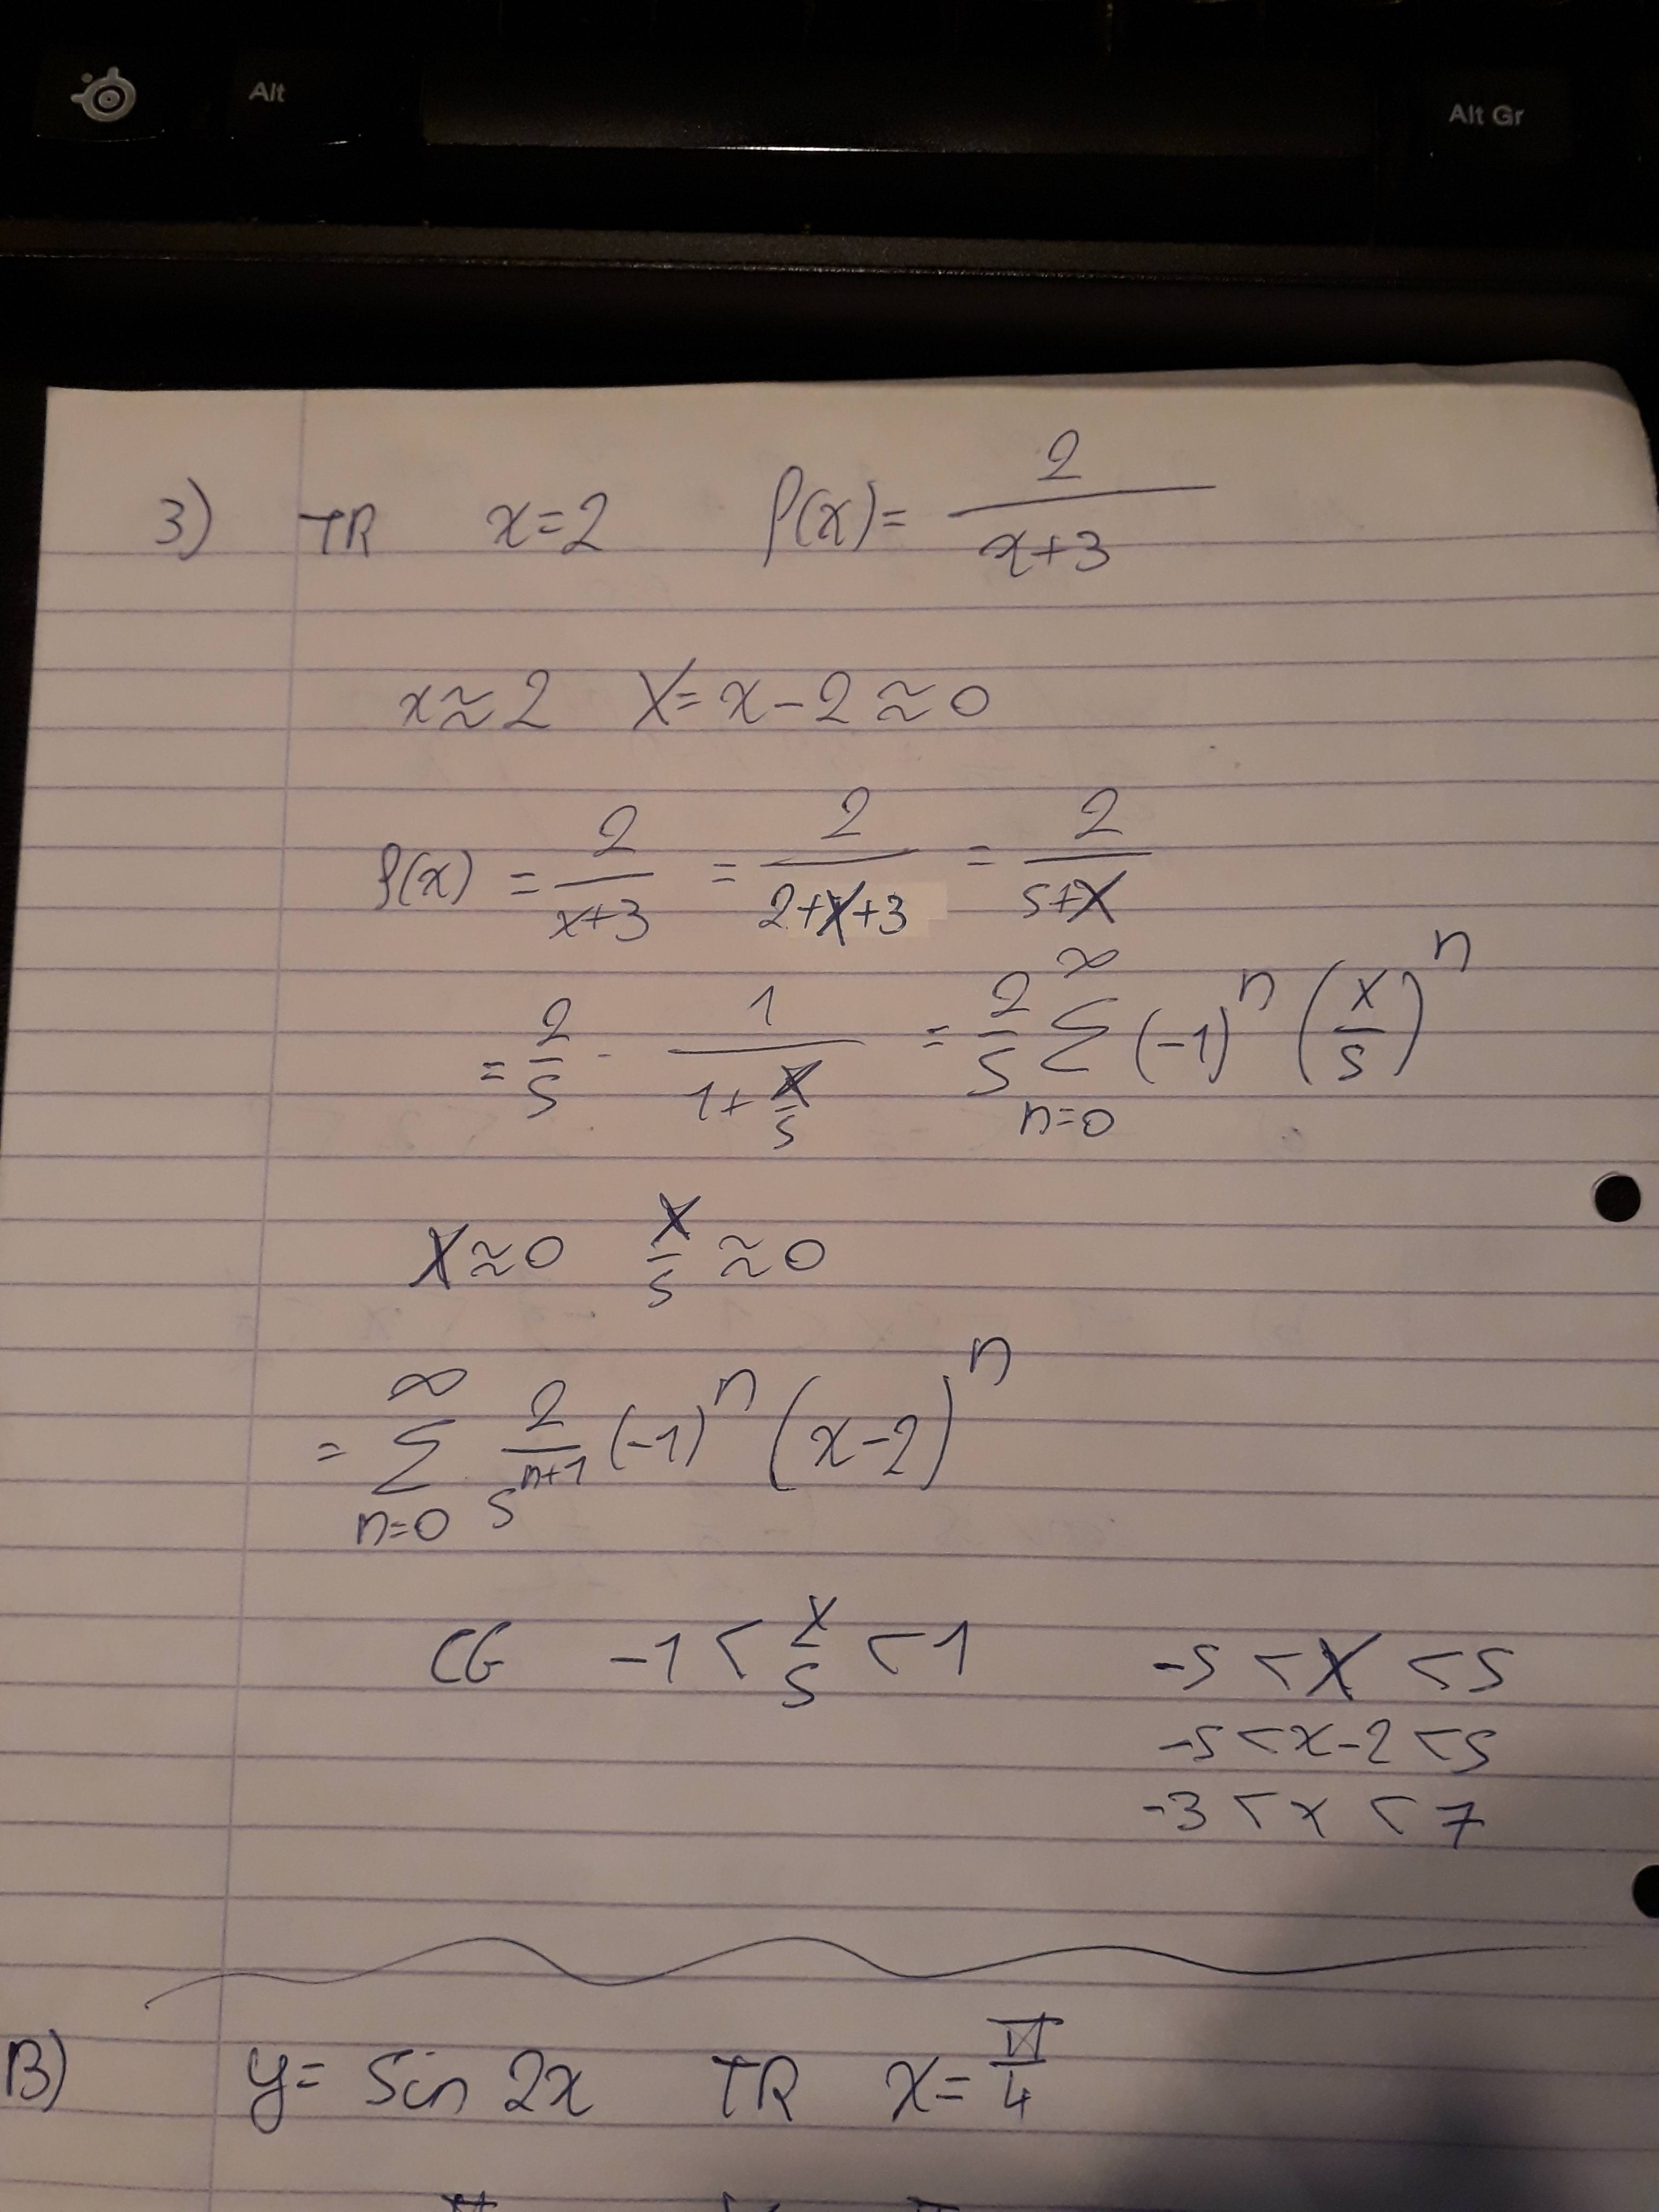
\includegraphics[width=\textwidth]{oef_3_taylor}
		\end{enumerate}
	}
\example{
    Ontwikkel $y = \sin 2x$ in een TR rond $x = \frac{\pi}{4}$ m.b.v. een bestaande Mc-Laurin reels
}{
    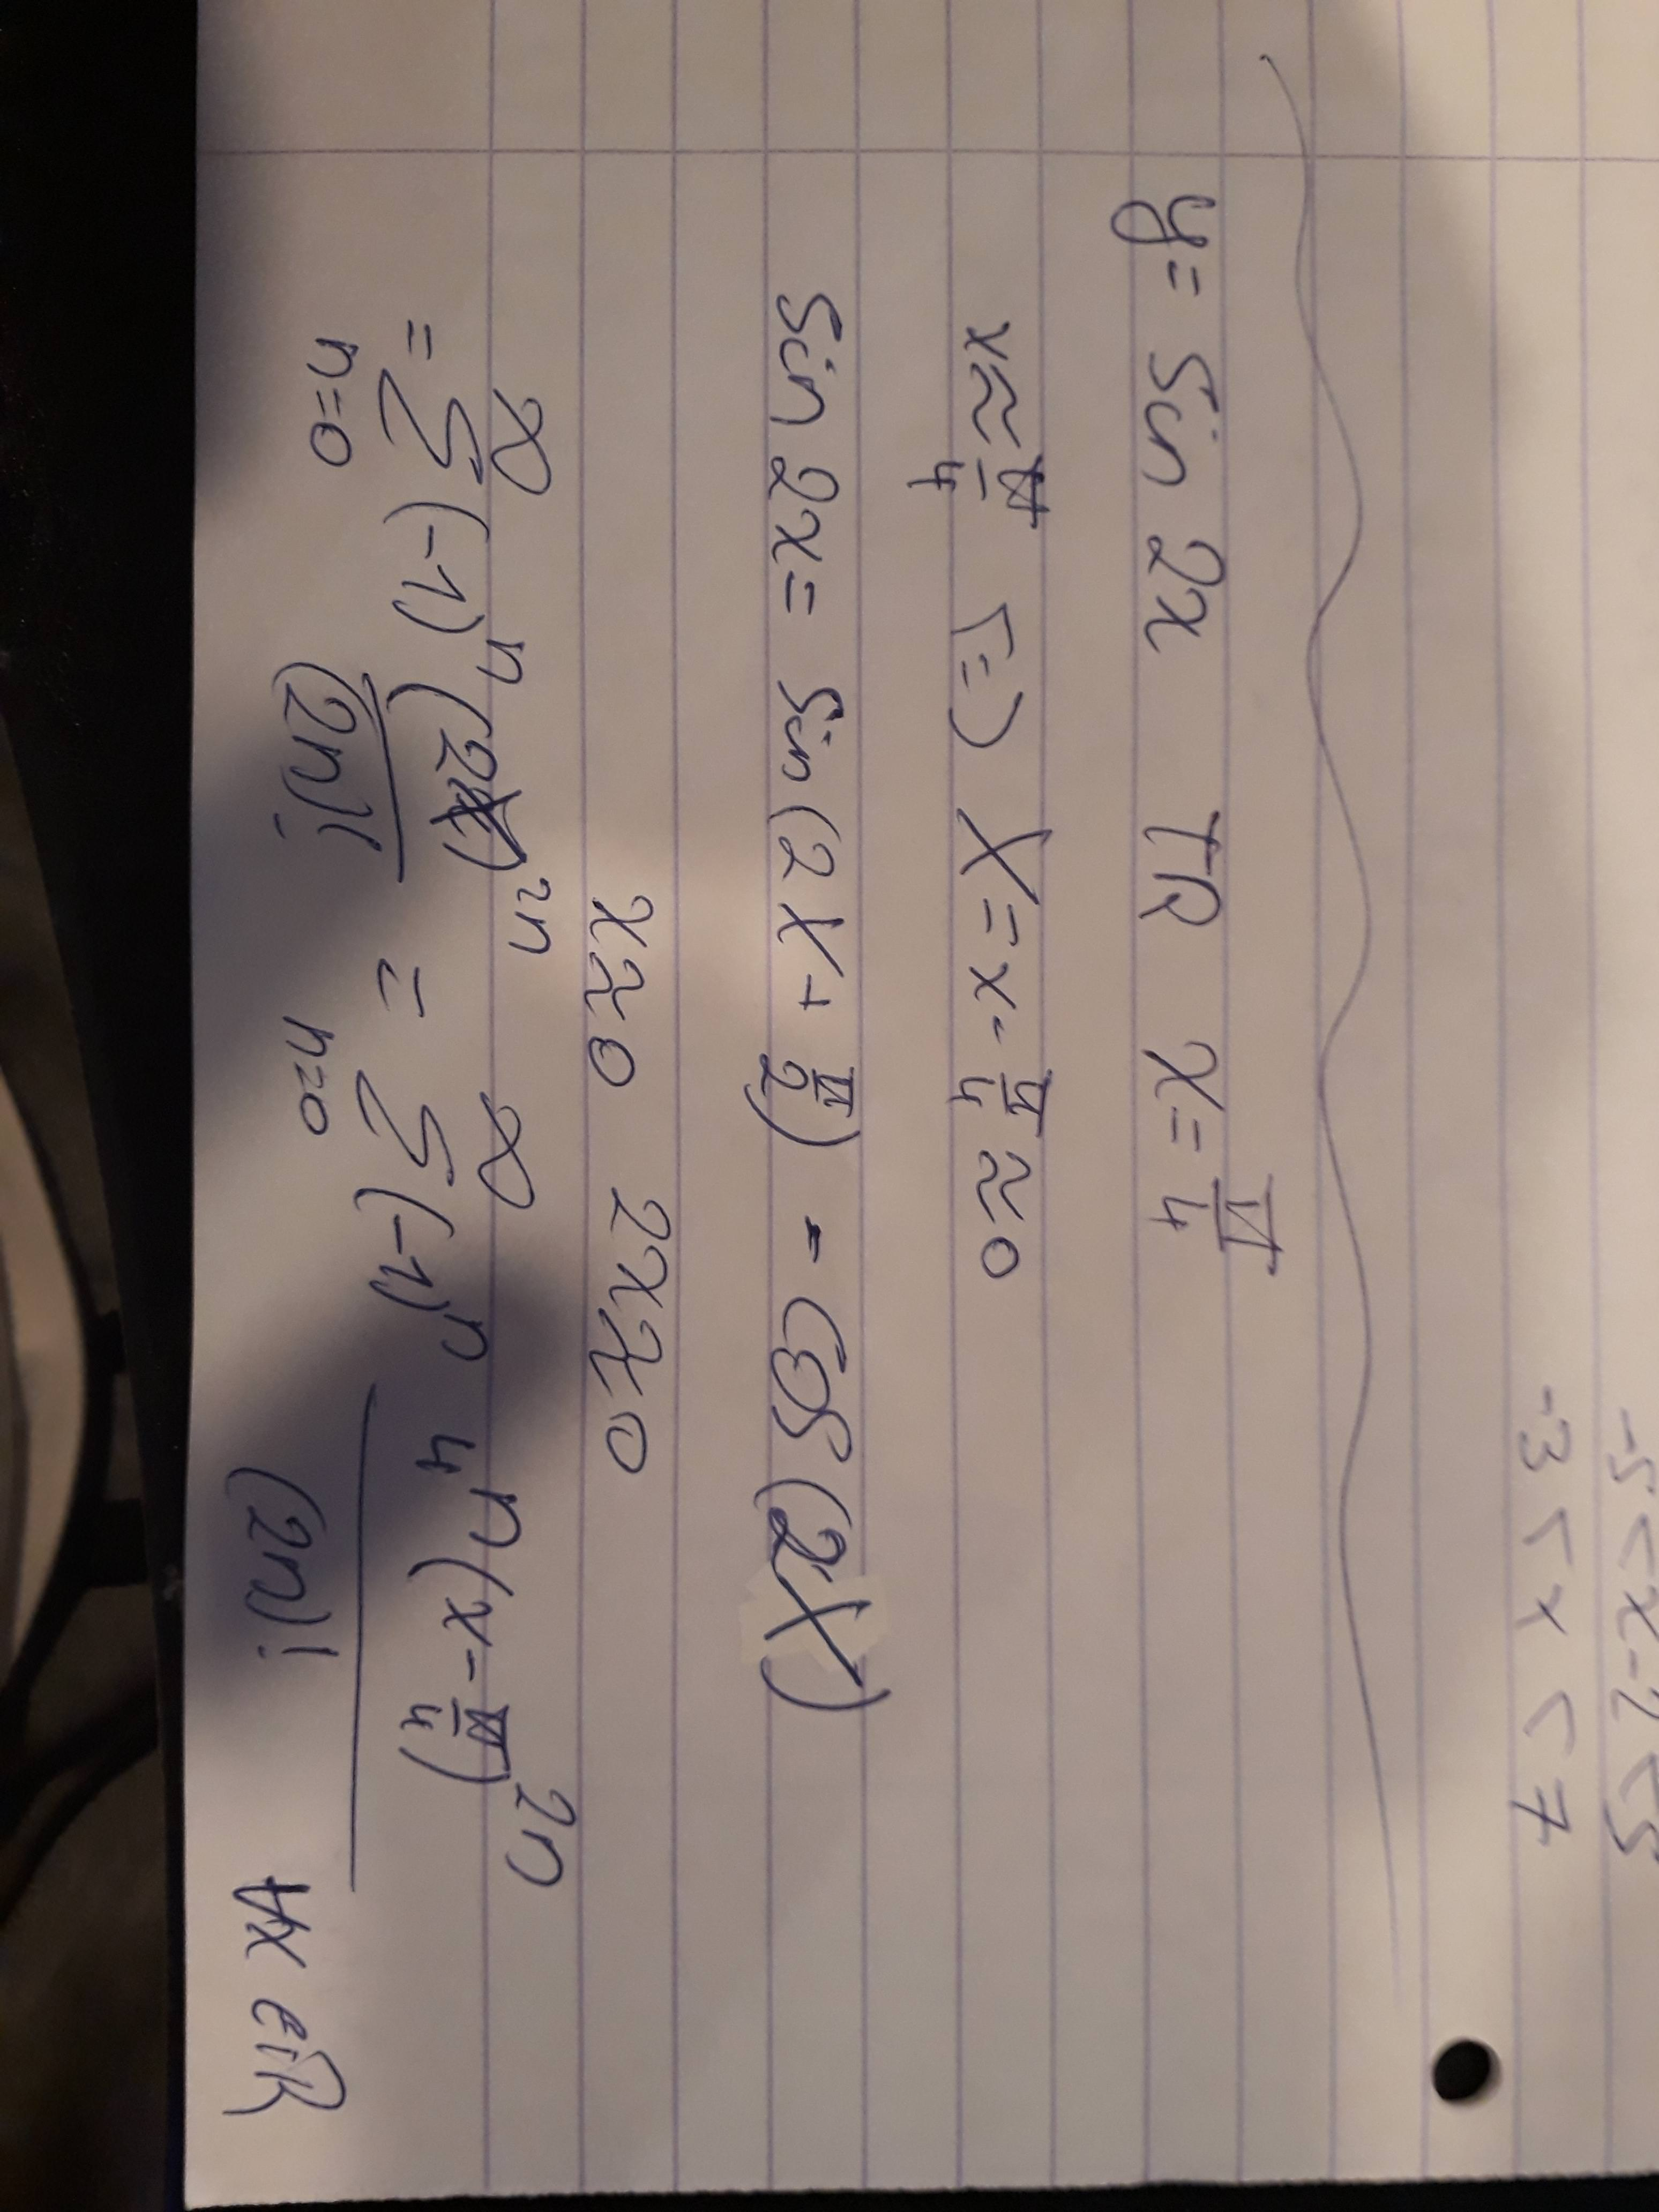
\includegraphics[width=0.7\textwidth, angle=90]{oef_b_taylor}
}

\example{
    Ontwikkel $y = (2x - 1)^2\ln(3x)$ in een TR rond $x = 1/2$ m.b.v. een bestaande Mc-Laurin reeks.
}{
    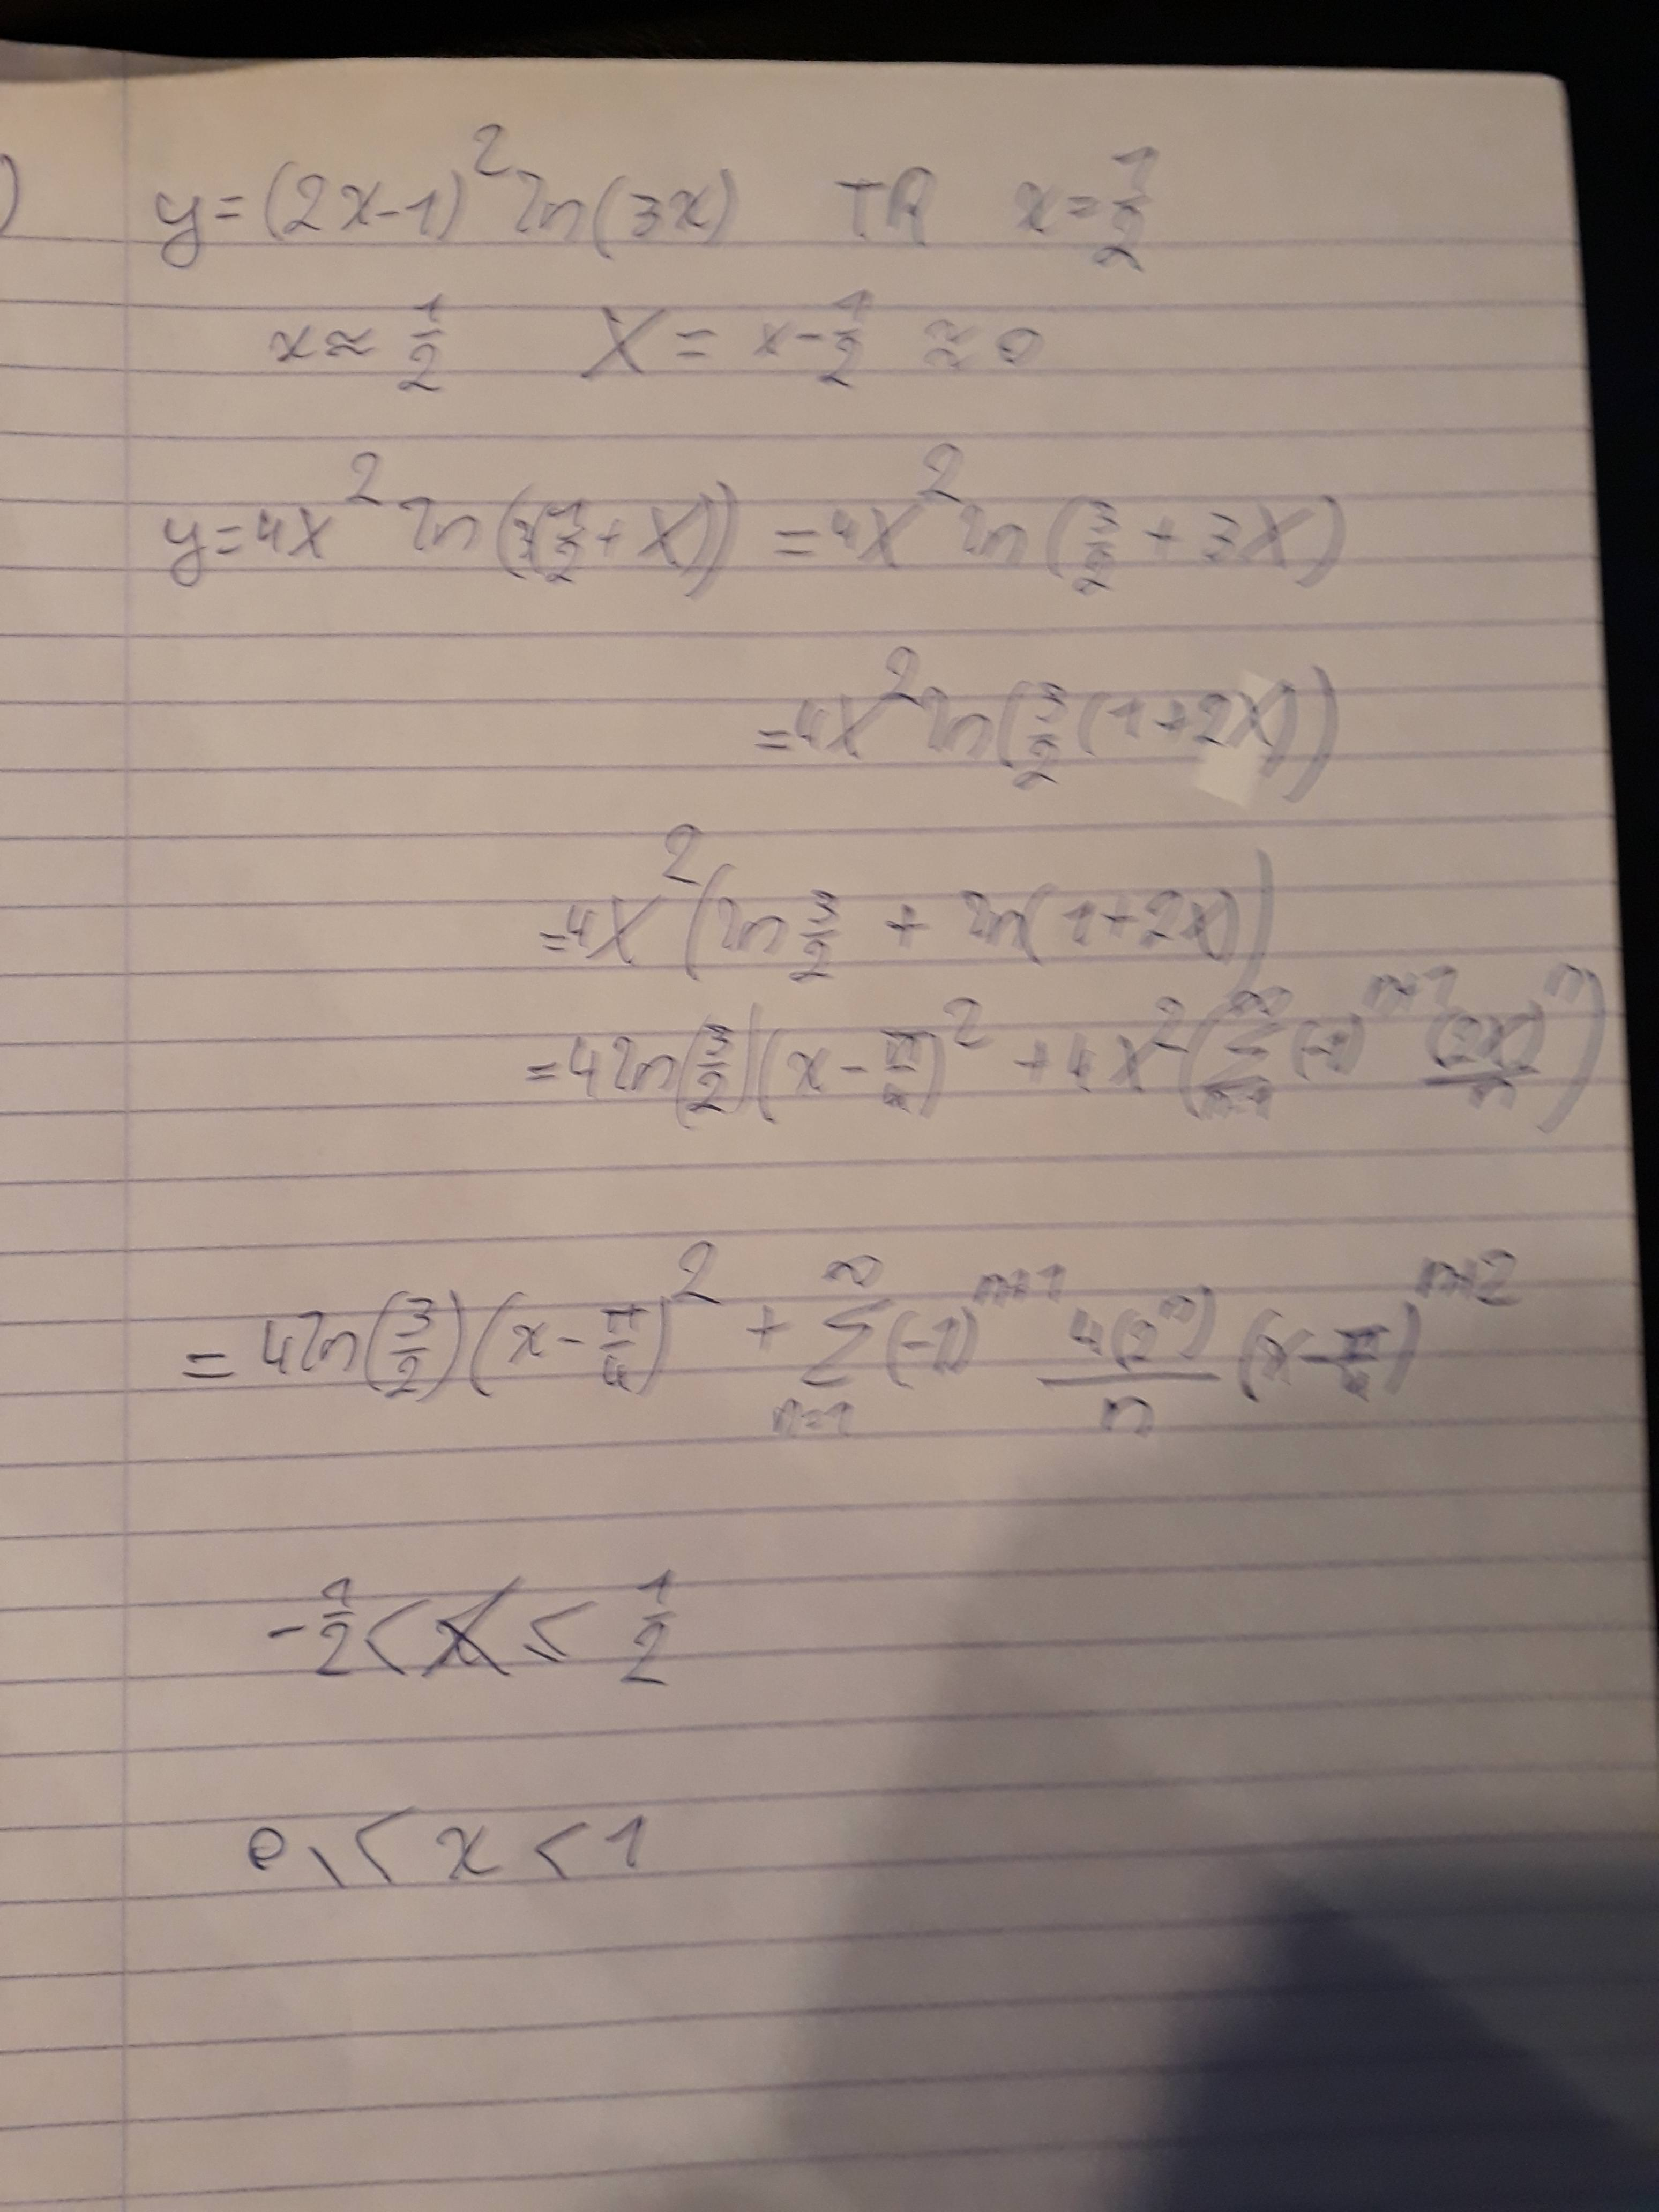
\includegraphics[width=\textwidth]{oef_c_taylor}
}
	\section{Fourrierreeksen}


	\example{
		Bepaal de fourierreeks horende bij:
		$$f(x) =    \begin{cases}
				0, -\pi < x < 0 \\
				x, 0 < x < \pi
			\end{cases}
			\qquad \hbox{met periode } 2\pi
		$$
	}{
		Aangezien de periode $2\pi$ is, wordt $L = \pi$. We bereken $a_0$, $a_k$ en $b_k$ apart.
		\begin{itemize}[label={}]
			\item   \begin{equation*}
				      \begin{split}
					      a_0 & = \frac{1}{\pi} \int_{-\pi}^{\pi} f(x)\;dx \\
					      & = \frac{1}{\pi}\bigg[\int_{-\pi}^{0} 0\;dx + \int_0^{\pi}x\;dx \bigg] \\
					      & = \frac{1}{\pi}\bigg[\frac{x^2}{2} \bigg]_{0}^{\pi} \\
					      & = \frac{\pi}{2}
				      \end{split}
			      \end{equation*}
			\item   \begin{equation*}
				      \begin{split}
					      a_k & = \frac{1}{\pi} \int_{-\pi}^{\pi} f(x)\cos \frac{k\pi x}{\pi} \;dx \\
					      & = \frac{1}{\pi} \bigg[0 + \int_0^{\pi}x\cos kx\;dx]\bigg] \\
					      & = \frac{1}{\pi} \bigg[\frac{x}{k}\sin(kx) + \frac{1}{k^2}\cos(kx)\bigg]_{0}^{\pi} \\
					      & = \frac{1}{\pi} \bigg[0 + \frac{1}{k^2}\cos(k\pi) - ( 0 + \frac{1}{k^2})\bigg] \\
					      & = \frac{1}{\pi k^2}(\cos(k\pi) - 1) \\
					      & = \frac{1}{\pi k^2}\big((-1)^k - 1 \big)
				      \end{split}
			      \end{equation*}
			      Indien $k \equiv 2k$ dan wordt $a_{2k} = 0$. Indien $k \equiv 2k + 1$ dan wordt $a_{2k + 1} = -\frac{2}{\pi(2k + 1)^2}$
			\item   \begin{equation*}
				      \begin{split}
					      b_k & = \frac{1}{\pi} \int_{-\pi}^{\pi} f(x)\sin kx \;dx \\
					      & = \frac{1}{\pi} \bigg[0 + \int_0^{\pi}x\sin kx\;dx]\bigg] \\
					      & = \frac{1}{\pi} \bigg[-\frac{x}{k}\cos(kx) + \frac{1}{k^2}\sin(kx)\bigg]_{0}^{\pi} \\
					      & = \frac{1}{\pi} \bigg[-\frac{\pi}{k}(-1)^k + 0 - ( 0 + 0)\bigg] \\
					      & = \frac{1}{\pi k^2}(-\frac{\pi}{k}(-1)^k) \\
					      & = -\frac{1}{k}(-1)^k \\
					      & = \frac{(-1)^{k + 1}}{k}
				      \end{split}
			      \end{equation*}
		\end{itemize}
		De fourierreeks wordt:
		$$\sum (x) = \frac{\pi}{4} + \sum_{k = 1}^{\infty} \bigg(-\frac{2}{\pi(2k + 1)^2}\cos[(2k + 1)x]  + \frac{(-1)^{k + 1}}{k}\sin kx\bigg)$$
	}

	\subsection{Belangrijke vereenvoudigingen}
	\begin{itemize}
		\item $f(x)$ even over een symmetrisch interval $[-a, a]:$
		      Bewijs zelf dat $b_k =0$ en de term $a_k$.
		\item $f(x)$ oneven over een symmetrisch interval $[-a, a]:$

		      $$a_k = \frac{1}{a}\int_{-a}^{a} f(x) \cos \frac{k\pi x}{a}\;dx = 0$$

		      $$b_k = \frac{1}{a}\int_{-a}^{a} f(x) \sin \frac{k\pi x}{a}\;dx = \frac{2}{a}\int_{0}^{a} f(x) \sin \frac{k\pi x}{a}\;dx $$

	\end{itemize}

	\example{
		Bepaal de fourierreeks horende bij
		$$f(x) = |x|$$
		over $[-1, 1]$
	}{
		We weten dat $2L = 2 \rightarrow L = 1$ en dat $b_k = 0$ want $f(x)$ is even over een symmetrisch interval. Berekening van $a_k$:
		\begin{equation*}
			\begin{split}
				a_k & = \int_{-1}^{1}|x|\cos k\pi x \; dx \\
				& = 2\int_0^1 x \cos k\pi x \; dx \\
				& = -\frac{4}{(2k + 1)^2\pi^2}
			\end{split}
		\end{equation*}
		Berekening van $a_0$
		\begin{equation*}
			\begin{split}
				a_0 & = 2\int_0^1 x \; dx \\
				& = 1
			\end{split}
		\end{equation*}
		De fourierreeks wordt:
		$$\sum (x) = \frac{1}{2} + \sum_{k = 0}^{\infty} - \frac{4}{(2k + 1)^2\pi^2}\cos[(2k + 1)\pi x]$$
	}

	\subsection{Opstellen van een Fourier-cosinusreeks voor f(x) over [a, b]}
	Maak een uitbreiding van de functie $f(x)$ zodat:
	$$f_E(x) = \begin{cases}
			f(x)  & x \in [a, b]   \\
			0     & x \in ]-a, a[  \\
			f(-x) & x \in [-b, -a]
		\end{cases}$$
	Aangezien $f_E(x)$ een even functie is over een symmetrisch interval wordt $b_k = 0$. Berekening van $a_k$:
	\begin{equation*}
		\begin{split}
			a_k & = \frac{1}{b} \int_{-b}^b f_E(x) \cos \frac{k\pi x}{b} \; dx \\
			& = \frac{2}{b} \int_0^b f_E(x)\cos \frac{k\pi x}{b} \; dx \\
			& = \frac{2}{b} \int_0^b f(x)\cos \frac{k\pi x}{b} \; dx \\
		\end{split}
	\end{equation*}

	\subsection{Opstellen van een Fourier-sinusreeks voor f(x) over [a, b]}
	Maak een uitbreiding van de functie $f(x)$ zodat:
	$$f_{OE}(x) = \begin{cases}
			f(x)   & x \in [a, b]   \\
			0      & x \in ]-a, a[  \\
			-f(-x) & x \in [-b, -a]
		\end{cases}$$
	Aangezien $f_{OE}(x)$ een oneven functie is over een symmetrisch interval wordt $a_k = 0$. Berekening van $b_k$: \todo{berekening}
\begin{equation*}
	\begin{split}
		b_k & = \frac{1}{b} \int_{-b}^b f_{OE}(x) \sin \frac{k\pi x}{b} \; dx \\
		& = ...
	\end{split}
\end{equation*}

\example{
	Stel $$f(x) =   \begin{cases}
			0     & 0 < x < 2 \\
			x^2   & 2 < x < 3 \\
			1 - x & 3 < x < 4
		\end{cases}$$
	Bepaal een uitbreiding over $[-4, 4]$ zodat
	\begin{enumerate}
		\item men een Fourier-sinusreeks bekomt
		\item men een Fourier-cosinusreeks bekomt
	\end{enumerate}
	Geef in beide gevallen de meest vereenvoudigde integralen die de coëfficiënten berekenen.
}{
	\begin{enumerate}
		\item Maak de uitbreiding: $$f_{OE} =   \begin{cases}
				      f(x)   & 0 < x < 4  \\
				      -f(-x) & -4 < x < 0
			      \end{cases}$$
		      Verder uitgeschreven:
		      $$f_{OE} =   \begin{cases}
				      f(x)   & 0 < x < 4   \\
				      -1 - x & -4 <x < -3  \\
				      -x^2   & -3 < x < -2 \\
				      0      & -2 < x < 0
			      \end{cases}$$
		      $f_{OE}(x)$ is een oneven functie over een symmetrisch interval dus $a_k = 0$. Opstellen van $b_k$:
		      \begin{equation*}
			      \begin{split}
				      b_k & = \frac{1}{4}\int_{-4}^4 f_{OE}(x)\sin \frac{k\pi x}{4}\; dx \\
				      & = \frac{1}{2} \bigg[\int_0^2 0\;dx + \int_2^3 x^2\sin \frac{k\pi x}{4} +\int_3^4 (1 - x)\sin \frac{k\pi x}{4}\bigg] \\
				      & = \frac{1}{2} \bigg[\int_2^3 x^2\sin \frac{k\pi x}{4} +\int_3^4 (1 - x)\sin \frac{k\pi x}{4}\bigg]
			      \end{split}
		      \end{equation*}
		\item Maak de uitbreiding
		      $$f_E(x) =  \begin{cases}
				      f(x)  & 0 < x < 4  \\
				      f(-x) & -4 < x < 0
			      \end{cases}$$
		      Verder uitgeschreven:
		      $$f_E(x) =  \begin{cases}
				      f(x)  & 0 < x < 4   \\
				      1 + x & -4 < x < -3 \\
				      x^2   & -3 < x < -2 \\
				      0     & -2 < x < 0
			      \end{cases}$$
		      $f_E(x)$ is een even functie over een symmetrisch interval dus $b_k = 0$. Opstellen van $a_k$:
		      \begin{equation*}
			      \begin{split}
				      a_k & = \frac{1}{4} \int_{-4}^4 f_E(x) \cos \frac{k\pi x}{4} \; dx\\
				      & = \frac{1}{2} \int_{0}^4 f(x) \cos \frac{k\pi x}{4} \;dx \\
				      & = \frac{1}{2}\bigg[\int_0^2 0\;dx + \int_{2}^{3} x^2\cos \frac{k\pi x}{4} + \int_{3}^4 (1 - x)\cos \frac{k\pi x}{4}\;dx \bigg] \\
				      & = \frac{1}{2}\bigg[\int_{2}^{3} x^2\cos \frac{k\pi x}{4} + \int_{3}^4 (1 - x)\cos \frac{k\pi x}{4}\;dx \bigg]
			      \end{split}
		      \end{equation*}
	\end{enumerate}
}


\example{
	\begin{enumerate}
		\item Bepaal de eerste van nul verschillende term in de Fourier-cosinusreeks over $[-4\pi, 4\pi]$ horende bij:
		      $$f(x) = \begin{cases}
				      -1, 0 < x < 2\pi   \\
				      2, 2\pi < x < 4\pi
                  \end{cases}$$
        \item Wat is de waarde van de fourierreeks in $x = 4\pi$ horende bij $f(x)$ gedefinieerd over $[0, 4\pi]$
        \item Wat is de waarde van de fourierreeks in $x = 4\pi$ horende bij de Fourier-cosinusreeks gedefinieerd over $[-4\pi, 4\pi]$ in $x = 4$
	\end{enumerate}
}{
	\begin{enumerate}
    \item Bepaal de Fourier-cosinusreeks door een uitbreiding te maken van $f(x)$.
        $$f_E(x) = \begin{cases}
            f(x) & 0 < x 4\pi \\
            f(-x) & -4\pi x < 0
        \end{cases}$$
    
        Bepaal $a_k$.
        \begin{equation*}
            \begin{split}
                a_k & = \frac{1}{4\pi} \int_{-4\pi}^{4\pi} f_E(x) \cos \frac{k\pi x}{4\pi} \; dx \\
                    & = \frac{2}{4\pi} \int_0^{4\pi} f(x)\cos \frac{kx}{4} \; dx \\
                    & = \frac{1}{2\pi}\bigg[\int_{0}^{2\pi} - 1 \cos \frac{kx}{4} \; dx + \int_{2\pi}^{4\pi} 2\cos \frac{kx}{4} \bigg] \\
            \end{split} 
        \end{equation*}
        Bepaal $a_0$.
        \begin{equation*}
            \begin{split}
                a_0 & = \frac{1}{2\pi}\bigg[\int_0^{2\pi} - 1 dx + \int_{2\pi}^{4\pi} 2\;dx  \bigg] \\
                    & =  \frac{1}{2\pi}\bigg[[-x]_0^{2\pi} + [2x]_{2\pi}^{4\pi} \bigg] \\
                    & = 1
            \end{split}
        \end{equation*}
    Bepaal de eerste van nul verschillende term.
    $$\sum (x) = \frac{1}{2} + ...$$
    \item   \begin{equation*}
                \begin{split}
                   \sum (4\pi)  & = \frac{1}{2}[f(4\pi) + f(0)] \\
                                & = \frac{1}{2}( 2 - 1) \\
                                & = \frac{1}{2} 
                \end{split}
            \end{equation*}
    \item   \begin{equation*}
                \begin{split}
                    \sum_E (4)  & = \frac{1}{2}[f_E(4^-) + f_E(4^+)] \\
                                & = \frac{1}{2}(-1 - 1) \\
                                & = -1
                \end{split}
            \end{equation*}
    \end{enumerate}     
}
